\documentclass[11pt,a4paper]{article}

\usepackage[utf8]{inputenc}
\usepackage[spanish]{babel}
\usepackage[T1]{fontenc}
\usepackage[margin=2.5cm]{geometry}
\usepackage{graphicx}
\usepackage{xcolor}
\usepackage{hyperref}

\hypersetup{colorlinks=true, urlcolor=blue, linkcolor=black}
\pagenumbering{gobble}

\begin{document}

\begin{center}
    {\Large\bfseries UNIVERSIDAD TÉCNICA ESTATAL DE QUEVEDO}\\[0.3em]
    {\large Facultad de Ciencias de la Ingeniería}\\
    {\large Carrera de Ingeniería de Software}\\[2em]

    {\huge\bfseries PRUEBA PRÁCTICA}\\[0.3em]
    {\huge\bfseries UNIDAD IV}\\[1em]
    {\large Ingeniería de Requisitos (ISR-401)}\\[3em]

    \begin{tabular}{ll}
        \textbf{Estudiante:} & Sánchez Centeno Roselyn Andreina \\[0.3em]
        \textbf{Curso:}      & 4to Software ``A'' \\[0.3em]
        \textbf{Asignatura:} & Ingeniería de Requisitos \\[0.3em]
        \textbf{Docente:}    & Ing. Gleiston Guerrero, Mg., PhD. \\[0.3em]
        \textbf{Fecha:}      & 11 de agosto de 2026 \\
    \end{tabular}

\end{center}

\vspace{2em}
\noindent\textbf{Link del repositorio:} \url{https://github.com/Roselyn15/Ev_Practica_Unidad_IV_RS}

\vspace{3em}
\begin{center}
    \large\textbf{Resumen del cuestionario (SGA)}
\end{center}

\begin{center}
    % Reemplazar por la captura real del resumen de resultados del cuestionario
    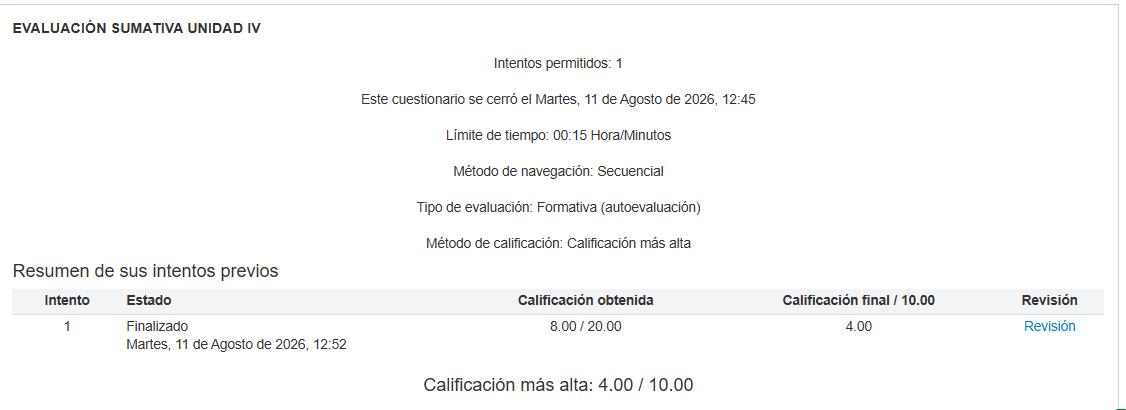
\includegraphics[width=0.85\textwidth]{capturas/resumen_cuestionario.png}
\end{center}

\vspace{2em}
\begin{center}
    \large\textbf{Captura de la evaluación / intento (SGA)}
\end{center}

\begin{center}
    % Reemplazar por la captura real de la evaluación/intento
    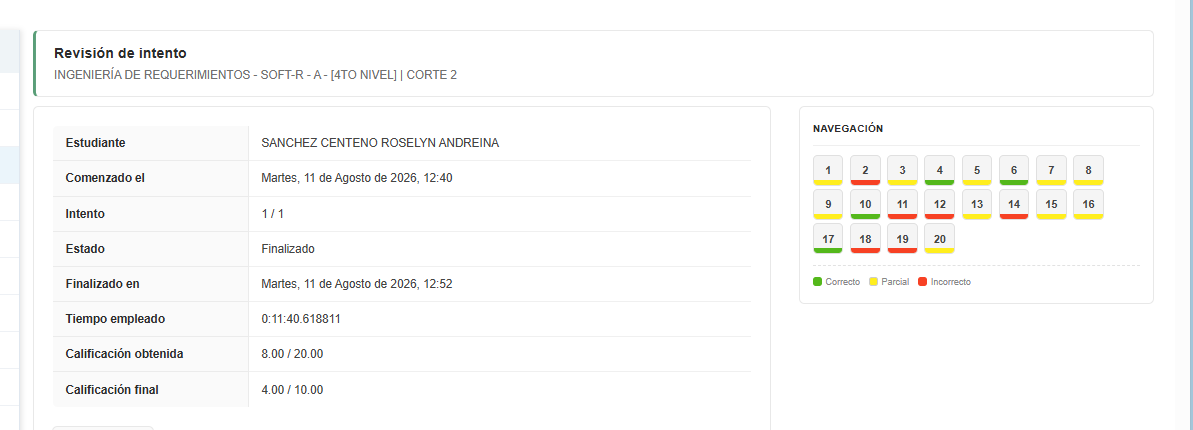
\includegraphics[width=0.85\textwidth]{capturas/evaluacion_intento.png}
\end{center}

\end{document}
